\documentclass[10pt]{beamer}

\mode<presentation>
{
  \usetheme[height=1.25cm]{Madrid}
  \setbeamertemplate{navigation symbols}{}
  \setbeamercolor{alerted text}{fg=illini}
}

\usebackgroundtemplate{
\includegraphics[width=\paperwidth,height=\paperheight]{uc-background}}

\usepackage[english]{babel}
\usepackage{epsfig,subfigure,bm}
\usepackage{multimedia}
\usepackage{psfrag}
\usepackage{animate}

%\usefonttheme{metropolis} % default family is serif
%%%%%% Begin of my macros and options

\setbeamertemplate{section in toc shaded}[default][55]
\setbeamertemplate{subsection in toc shaded}[default][55]
\setbeamercolor{block title}{fg=white,bg=illini}
\setbeamercolor{block body}{fg=black,bg=mygrey}

\setbeamercolor{emphprimary}{fg=CBlue}
\setbeamercolor{emphsecondary}{fg=illini}
\setbeamercolor{emphtertiary}{fg=mygreen}
\definecolor{darkForestGreen}{rgb}{.1,1,.1}
\definecolor{veryLightGray}{rgb}{.9,.9,.9}
\definecolor{greenApple}{rgb}{.3,.9,.3}

\setbeamercolor{frametitle}{bg=CBlue}   
\setbeamercolor{title}{bg=CBlue}

\usepackage{amsmath,amssymb,amsxtra,amsthm}
\usepackage{algorithm,algorithmic}
\usepackage{natbib}
\usepackage{bibentry}
\usepackage{xspace}
\usepackage{changepage}

\definecolor{myblue}{rgb}{.2,.2,.7}
\definecolor{myred}{rgb}{.7,.2,.2}
\definecolor{mygreen}{rgb}{.2,.7,.2}
\definecolor{mygrey}{rgb}{0.9,0.9,0.9}
\definecolor{CBlue}{cmyk}{1,0.25,0,0}
\definecolor{illini}{rgb}{0.98,0.4,0.05}
\definecolor{black}{cmyk}{0,0,0,1}

\newcommand{\myemph}[1]{{\usebeamercolor[fg]{emphprimary}
    \textbf{#1}}}
\newcommand{\myemphalt}[1]{{\usebeamercolor[fg]{emphsecondary}
    \textbf{#1}}}

\graphicspath{{figs/}}

\title[Math for Robotics] % (optional, use only with long paper titles)
{CSE276C - Integration of ODEs}

\author[H.~I. Christensen] % (optional, use only with lots of authors)
{Henrik I.~Christensen}
% - Give the names in the same order as the appear in the paper.  -
% Use the \inst{?} command only if the authors have different
% affiliation.

\AtBeginSection[]
{
   \begin{frame}
       \frametitle{Outline}
       \tableofcontents[currentsection]
   \end{frame}
}

\institute[UCSD] % (optional, but mostly needed)
{
  \begin{minipage}[c]{.2\textwidth}
    
\includegraphics[width=.65\linewidth]{ucsealnew}%
  \end{minipage}%
  \begin{minipage}[c]{.6\textwidth}
    \small
%%    \begin{center}
      Computer Science and Engineering\\
      University of California, San Diego\\
      \myemph{\url{http://cri.ucsd.edu}}\\          
%%    \end{center}

  \end{minipage}
%%  \vspace*{1ex}
}
%% - Use the \inst command only if there are several affiliations.
%% - Keep it simple, no one is interested in your street address.

\bigskip

\date[Oct 2020]% (optional, should be abbreviation of conference name)
{\small%
  October 2020}

\begin{document}
  
\nobibliography{/Users/hic/Dropbox/bibliography/bib-file}
\bibliographystyle{plain}

\begin{frame}[plain]
  \titlepage
\end{frame}

\begin{frame}
  \frametitle{Literature }
  \begin{itemize}
  \item Numerical Recipes: Chapter 16
  \item Numerical Renaissance: Chapter 9
  \end{itemize}
\end{frame}

\section{Introduction}

\begin{frame}
  \frametitle{Introduction}
  \begin{itemize}
  \item For integration of a set of ordinary differential equations
    you can always reduce it into a set of first order differential
    equations. 
  \item Example
    \[
      \frac{d^2 y}{d x^2} + q(x) \frac{dy}{dx} = r(x)
    \]
  \item which can be rewritten
    \[
      \begin{array}{rcl}
        \frac{dy}{dx} & = & z(x)\\
        \frac{dz}{dx} & = & r(x)  - q(x) z(x) \\
      \end{array}
    \]
  \item where z is a new variable
  \end{itemize}  
\end{frame}

\begin{frame}
  \frametitle{Small example}
  \begin{itemize}
  \item Consider a simple motion of a mass when actuated by a mass
    \[
      F(u_1) = m \frac{ d^2 u_1 }{ d t^2 }
    \]
  \item We can rewrite this as
    \[
      \frac{d^2 u_1}{d t^2} = \frac{1}{m} F(u_1)
    \]
  \item We can introduce $u_2 = \frac{du_1}{dt}$ to generate
    \[
      \begin{array}{rcl}
        \frac{du_1}{dt} & = & u_2\\
        \frac{du_2}{dt} & = & \frac{1}{m} F(u_1)
      \end{array}
    \] OR
    \[
      \frac{du}{dt} = f( u, t) \mbox{~~~~ with ~~~~} u = \left(
        \begin{array}{c}
          u_1 \\ u_2\\
        \end{array} \right)
    \]
    where
    \[
      f = \left(
        \begin{array}{c}
          u_2\\
          \frac{F(u_1)}{m}\\
        \end{array} \right)
    \]
  \end{itemize}
\end{frame}

\begin{frame}
  \frametitle{Introduction (cont)}
  \begin{itemize}
  \item The generic problem is thus a set of couple 1st order differential equations
    \[
      \frac{d y_i(x)}{dx} = f_i(x_i, y_1, y_2, \ldots, y_n)
    \]
  \item There are three major approaches:
    \begin{enumerate}
    \item Runge-Kutta: Euler type propagation
    \item Richardson extrapolation / Burlirsch-Stoer: extrapolation type estimation with small step sizes
    \item Predictor-Corrector: extrapolation with correction. 
    \end{enumerate}
  \item Runge-Kutta most widely adopted for ``generic'' problems. Great if function evaluation is cheap
  \item Burlirsch-Stoer generates higher precision
  \item Predictor-Corrector is historically interesting, but rarely used today
  \end{itemize}
\end{frame}

\section{Runge-Kutta}

\begin{frame}
  \frametitle{Runge-Kutta}
  \begin{itemize}
  \item The forward Euler method is specified as
    \[
      y_{n+1} = y_n + h f( x_n, y_n )
    \]
    with $x_{n+1} = x_n + h$ 
  \item A problem is that the integration is asymmetric
    \centerline{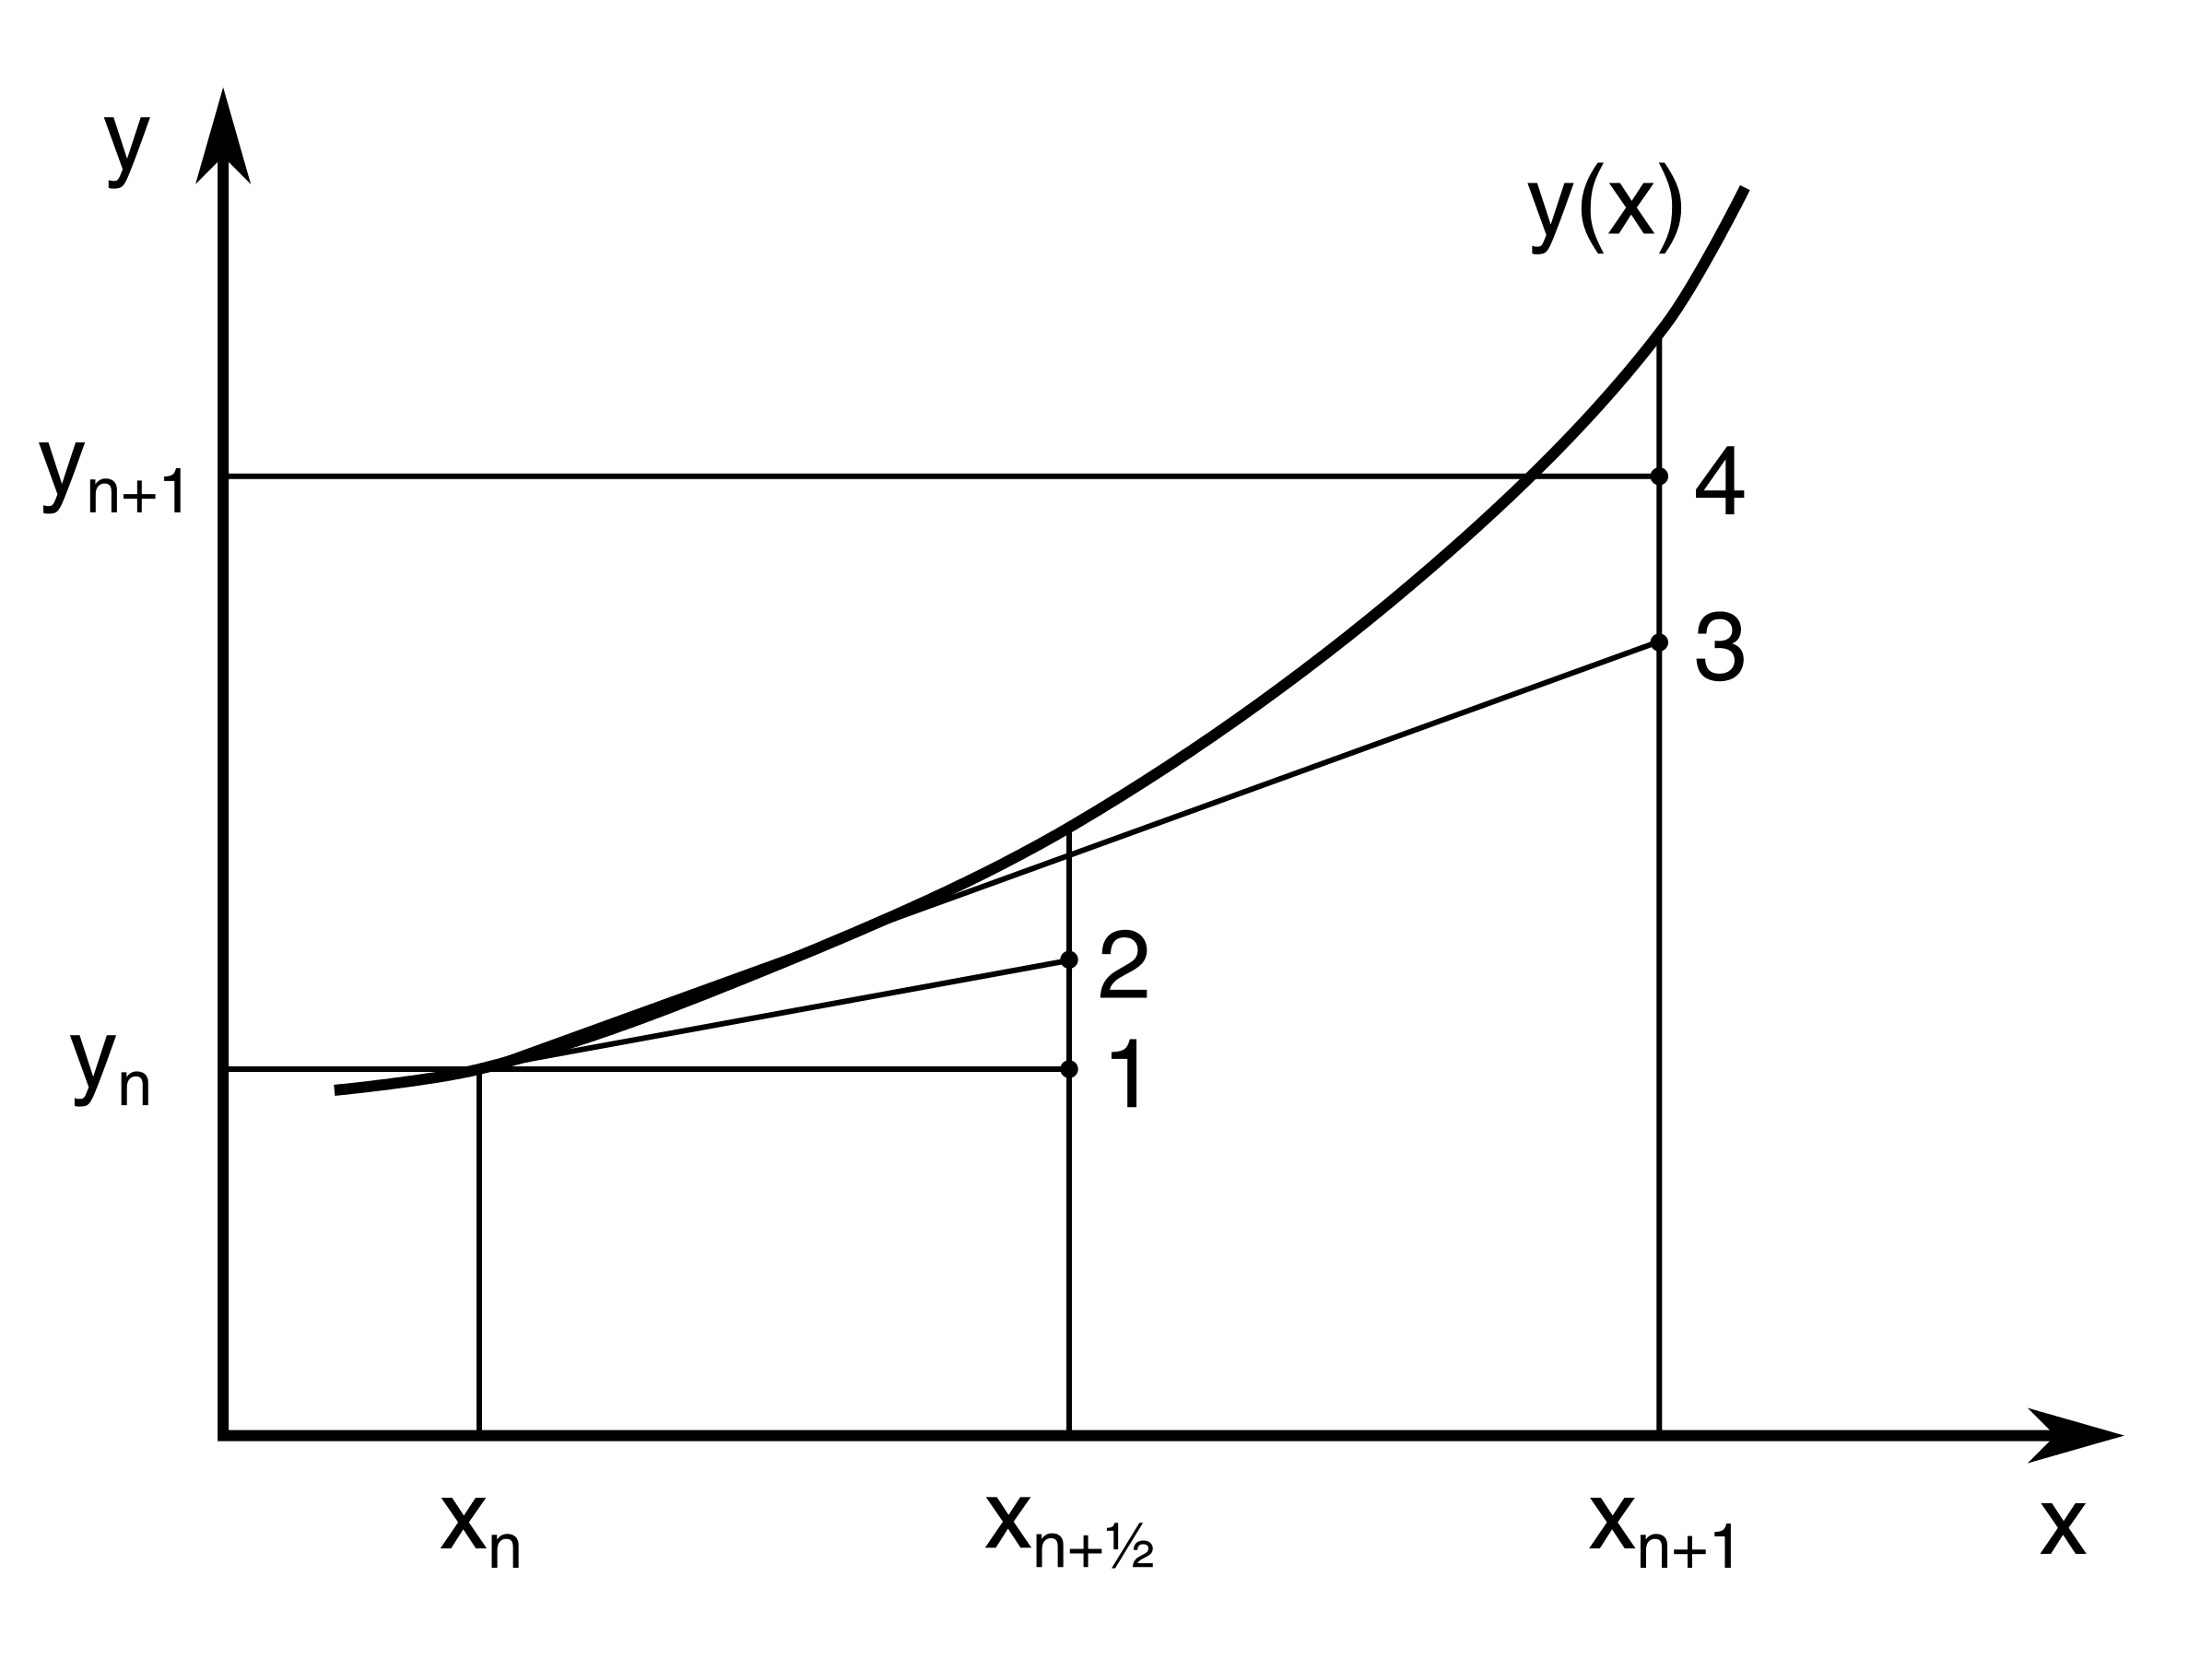
\includegraphics[height=5cm]{12}}
  \end{itemize}
\end{frame}

\begin{frame}
  \frametitle{Runge-Kutta - Stepped Up}
  \begin{itemize}
  \item We can use a mid-point to get a closer estimate, i.e.,
    \[
      \begin{array}{rcl}
        k_1 & = & h f(x_n, y_n)\\
        k_2 & = & h f( x_n + \frac{1}{2} h, y_n + \frac{1}{2} k_1)\\
        y_{n+1} & = & y_n + k_2 + O(h^3)\\
      \end{array}
    \]
  \end{itemize}
\end{frame}

\begin{frame}
  \frametitle{4th order Runge-Kutta}
  \begin{itemize}
  \item We can easily extend to richer models. A typical example is the fourth order model
    \[
      \begin{array}{rcl}
        k_1 & = & h f( x_n, y_n)\\
        k_2 & = & h f( x_n + \frac{1}{2} h, y_n + \frac{1}{2} k_1)\\ 
        k_3 & = & h f( x_n + \frac{1}{2} h, y_n + \frac{1}{2} k_2)\\
        k_4 & = & h f( x_n + h, y_n + k_3)\\
        y_{n+1} & = & y_n + \frac{1}{6} k_1 + \frac{1}{3} k_2 + \frac{1}{3} k_3 + \frac{1}{6} k_4 + O(h^5)\\        
      \end{array}
    \]
  \item By far the most frequently used RK method for ODE integration
  \item Requires four function evaluations for every step
  \end{itemize}
\end{frame}

\begin{frame}
  \frametitle{Adaptive Runge-Kutta}
  \begin{itemize}
  \item Could we adjust the step-size? 
  \item Estimation of performance adds an overhead
  \item What would be an obvious solution? \pause
    \begin{enumerate}
    \item Do a full step
    \item Do a half step
    \item Compare (could be recursive)
    \item Next
    \end{enumerate}
  \item In general no one goes beyond 5th order Runge-Kutta
  \end{itemize}
\end{frame}

\begin{frame}
  \frametitle{PI step control of RK}
  \begin{itemize}
  \item Could we use PI control to track stepsize? \pause
  \item How about
    \[
      h_{n+1} = S h_n \mbox{err}_n^{\alpha} \mbox{err}_{n-1}^{\beta}
    \]
    where S is a scale factor. $\alpha$ and $\beta$ are gain factors
  \item Typical default values $\alpha$ = $\frac{1}{k} - 0.75 \beta$
    and $\beta = \frac{0.4}{k}$ and k is an integer that designates
    order of the integrator
  \end{itemize}
\end{frame}
\section{Richardson / Burlirsch-Stoer}

\begin{frame}
  \frametitle{Richardson Extrapolation / Burlirsch-Stoer}
  \begin{itemize}
  \item Aimed at smooth functions 
  \item Generates best precision with minimal effort
  \item Things to consider
    \begin{enumerate}
    \item Does not do well on functions w. table lookup or interpolation
    \item Not well suited for functions with singulaties within intg range
    \item Not well suited for ``expensive'' functions
    \end{enumerate}
  \item The approach is based on three ideas
    \begin{enumerate}
    \item Final answer is based on selection of (adaptive) stepsize just like Romberg
    \item Use of rational functions for extrapolation (allow larger h)
    \item Integration method reply on use of even functions
    \end{enumerate}
  \item Typically the steps size H is large and h is 100+ steps
  \end{itemize}
\end{frame}

\begin{frame}
  \frametitle{Burlirsch-Stoer - The details}
  \begin{itemize}
  \item Consider a modified mid-point strategy
    \[
      x_{n+1} = x_n + H
    \] but with sub-steps
    \[
      h = \frac{H}{n}
    \]
  \item We can rewrite the integration
    \[
      \begin{array}{rcl}
        z_0 & = & y(x_n)\\
        z_1 & = & z_0 + h f( x_n, z_0 )\\
        z_{m+1} & = & z_{m-1} + 2h f(x_{n} + mh, z_n) \mbox{~~~} m = 1, 2, 3, ...{n-1}\\
        y(n_n + H) & = & \frac{1}{2} [ z_n + z_{n-1} + h f(x+H, z_n) ] \\ 
      \end{array}
    \]
  \item Centered mid-point or centered difference method
  \item The error can be shown to be
    \[
      y_n - y(x+H) = \sum_{i=0}^{\infty} \alpha_i h^{2i}
    \]
  \item The power series implies that we can potentially do less evaluation. 
  \end{itemize}
\end{frame}

\begin{frame}
  \frametitle{Burlirsch-Stoer - How good is it? }
  \begin{itemize}
  \item Suppose n is even and $y_{n/2}$ is the results of half as many steps    
  \item Then
    \[
      y(x+H) = \frac{4 y_n - y_{n/2}}{3}
    \]
  \item which is arccurate to the 4th order as Runge-Kutta but with
    2/3 less derivative evaluation? 
  \item How do you choose good step sizes for refinement? \pause
  \item One strategy could be
    \[
      n = 2, 4, 6, 8, 12, 16, 24, 32, \ldots \mbox{~~~~} n_ = 2 n_{j-2}
    \]
    more recently a suggestion
    \[
      n - 2, 3, 6, 8, 10, 12, 14, \ldots \mbox{~~~~} n_j = 2(j+1)
    \]
  \end{itemize}  
\end{frame}

\begin{frame}
  \frametitle{Step size control for Burlirsch-Stoer}
  \begin{itemize}
  \item The error estimate can be tabulated as
    \[
      \begin{array}{lll}
        T_{00} && \\
        T_{10} & T_{01} & \\
        T_{20} & T_{11} & T_{22} \\
      \end{array}
    \]
  \item where $T_{ij}$ is the Lagrange interpolation of order i with j points. The relation between the polynomials is
    \[
      T_{k, j+1} = \frac{2 T_{k,j} - T_{k-1,j}}{(n_k / n_{k-j-1})^2 - 1} \mbox{~~~~} j = 0, 1, \ldots, k-1
    \]
  \item Each stepsize starts a new row. The difference
    $T_{kk} - T_{kk-1}$ is an an error estimate
  \item We can pre-compute the error estimates and use them to decide
    on step-size selection
  \end{itemize}
\end{frame}


\section{Variable Dynamics}

\begin{frame}
  \frametitle{Variable Dynamics}
  \begin{itemize}
  \item Sometimes the variable dynamics are very different
  \item Consider
    \[
      \begin{array}{rcl}
        u' & = & 998 u + 1998 v\\
        v' & = & -999u - 1999 v\\
      \end{array}
    \]
  \item with u(0) = 1 and v(0) = 0 we can get
    \[
      \begin{array}{rcl}
        u = 2 y - z & \mbox{~~~}& v = -y -z \\
      \end{array}
    \]
    We can solve and find
    \[
      \begin{array}{rcl}
        u & = & 2 e^{-x} - e^{-1000x}\\
        v & = & - e^{-x} + e^{-1000x}\\
      \end{array}
    \]
  \item The differneces in dynamics would generate challenging step sizes
  \end{itemize}
\end{frame}

\section{Partial Differential Equations}
\label{sec:part-diff-equat}

\begin{frame}
  \frametitle{Partial Differential Equations}
  \begin{itemize}
  \item Huge topics that has its own course - MATH 110/MATH 231 A-C
  \item Widely used for studies of physical systems - simulation / analysis
  \item Three main categories
    \begin{enumerate}
    \item Hyperbolic (wave equation)
      \[
        \frac{\partial^2 u}{\partial t^2} = v^2 \frac{\partial^2 u}{\partial x^2}
      \] where v is the speed of wave propagation
    \item Parabolic (diffusion equation)
      \[
        \frac{\partial u}{\partial t} = \frac{\partial}{\partial x}\left( D \frac{\partial  u}{\partial x} \right)
      \]
      where D is the diffusion coefficient
    \item Elliptic (Poisson equation)
      \[
        \frac{\partial^2 u }{\partial x^2} +  \frac{\partial^2 u }{\partial y^2} = \rho(x,y)
      \]
      where $\rho()$ is the source term. 
    \end{enumerate}
  \end{itemize}
\end{frame}

\begin{frame}
  \frametitle{Computational Considerations for PDEs}
  \begin{center}
    \begin{tabular}{cc}
      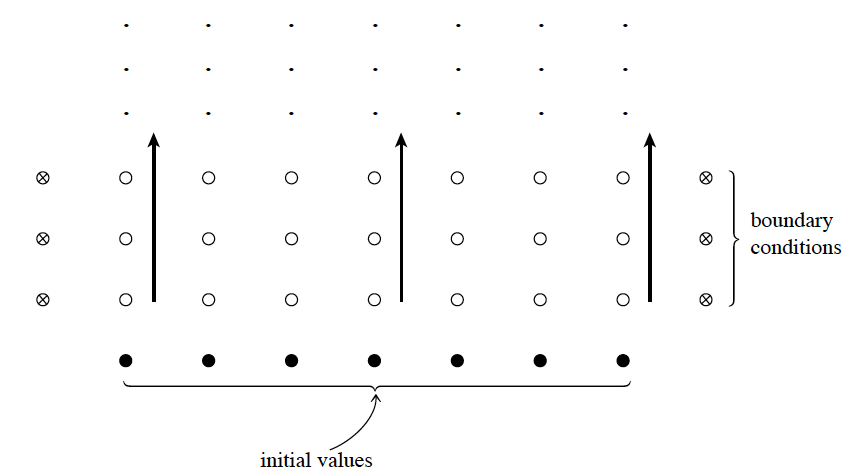
\includegraphics[height=3cm]{initial-value}&
      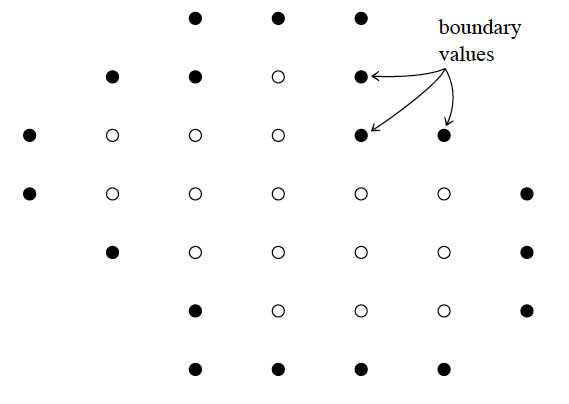
\includegraphics[height=3cm]{boundary-value}\\
      Initial Value & Boundary Value\\
    \end{tabular}  
  \end{center}

  ~\\[1cm]
  Source - Numerical Recipes. 
\end{frame}

\begin{frame}
  \frametitle{Finite difference calculations}
  \begin{columns}
    \begin{column}{7cm}
      \begin{itemize}
      \item In most cases grid propagation
      \item Finite differences is a basic approximation
      \item Final structure is a sparse matrix 
      \item Numerous models and packages to address
      \end{itemize}
    \end{column}
    \begin{column}{4cm}
      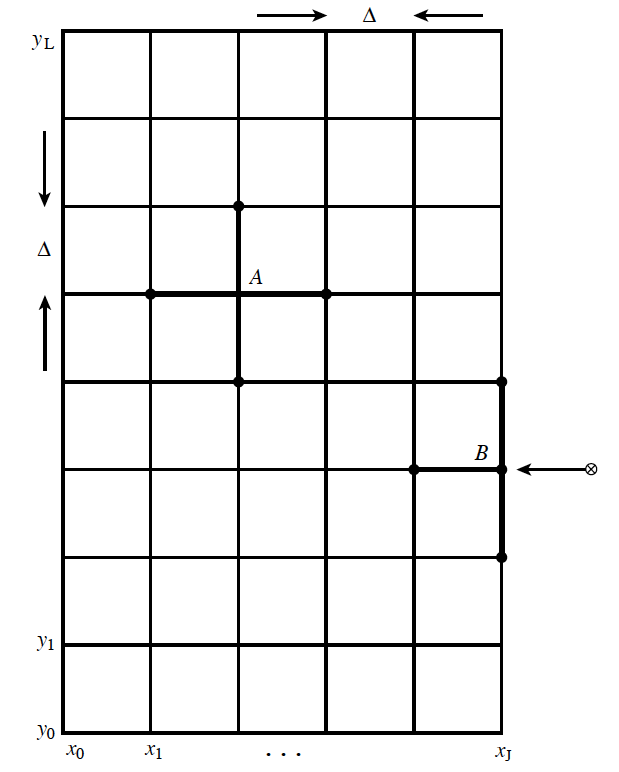
\includegraphics[width=3.5cm]{finite-differences}
    \end{column}
  \end{columns}
\end{frame}


\section{Summary}

\begin{frame}
  \frametitle{Summary}
  \begin{itemize}
  \item We can organize ODEs as a set of coupled 1st order ODEs
  \item Runge-Kutta is ideal for ``cheap'' functions, especially 4th
    order approximation
  \item Buerlirsch-Stoer is ideal for high-accuracy integration
  \item It is important to consider the variable dynamics in
    integration of functions.
  \item Adaptive stepsize is often valuable as a way to generate
    realistic complexity
  \end{itemize}
\end{frame}

\end{document}

%%% Local Variables:
%%% mode: latex
%%% TeX-master: t
%%% End:
